\documentclass[11pt]{article}
\usepackage{pgfplots}
\usepackage{tikz}
\usetikzlibrary{positioning,calc}
\pgfplotsset{compat=1.18}

\usepackage[margin=1in]{geometry}
\usepackage{graphicx}

\title{MATILDA Scalability Analysis}
\author{Generated from scalability\_summary.json}
\date{\today}

\begin{document}

\maketitle

\section{Scalability Results}

This document presents scalability test results for MATILDA TGD discovery system.

\textbf{Configuration:}
\begin{itemize}
    \item Algorithm: astar
    \item Heuristic: hybrid
    \item Max N: 3
    \item Max Variables: 6
\end{itemize}

\subsection{Runtime Scaling}

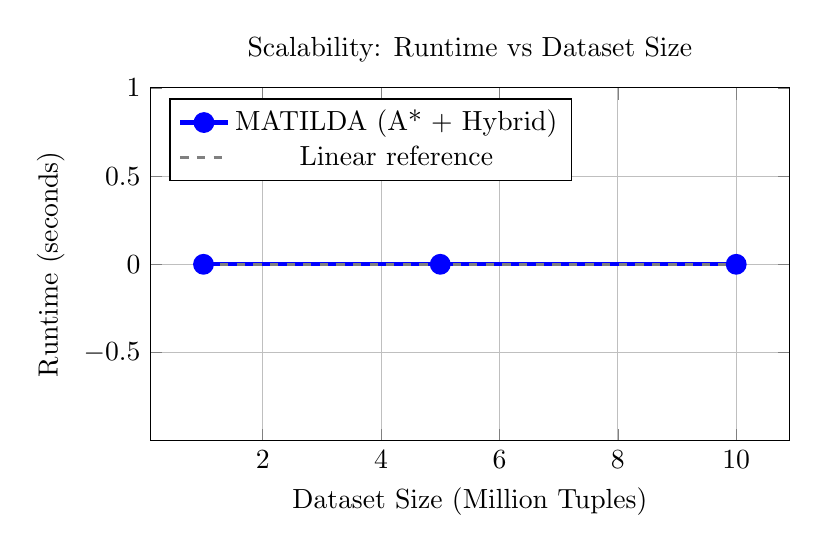
\begin{tikzpicture}
\begin{axis}[
    width=0.8\textwidth,
    height=0.5\textwidth,
    xlabel={Dataset Size (Million Tuples)},
    ylabel={Runtime (seconds)},
    title={Scalability: Runtime vs Dataset Size},
    grid=major,
    legend pos=north west,
    ymajorgrids=true,
    xmajorgrids=true,
    mark size=3pt,
]

% MATILDA data
\addplot[
    color=blue,
    mark=*,
    line width=1.5pt,
] coordinates {
    (1.0,0.00)
    (5.0,0.00)
    (10.0,0.00)
};
\addlegendentry{MATILDA (A* + Hybrid)}

% Linear reference
\addplot[
    color=gray,
    dashed,
    line width=1pt,
] coordinates {
    (1.0,0.00)
    (5.0,0.00)
    (10.0,0.00)
};
\addlegendentry{Linear reference}

\end{axis}
\end{tikzpicture}


\subsection{Rules Discovery}

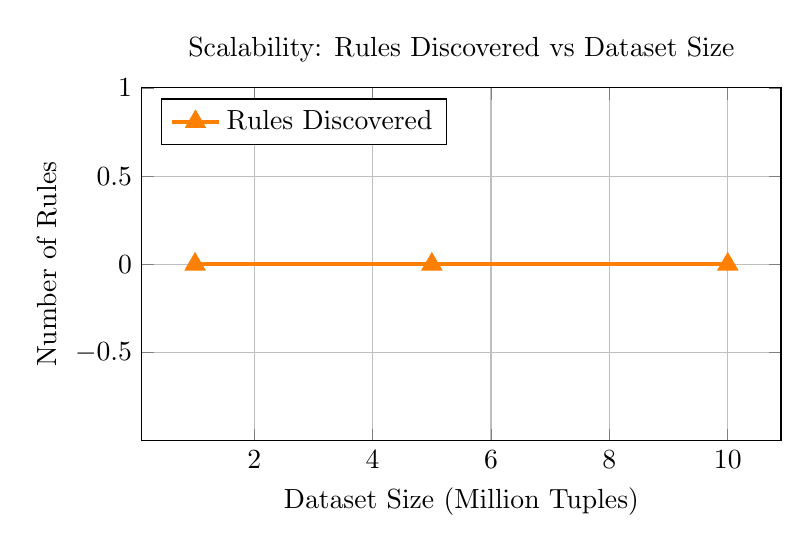
\begin{tikzpicture}
\begin{axis}[
    width=0.8\textwidth,
    height=0.5\textwidth,
    xlabel={Dataset Size (Million Tuples)},
    ylabel={Number of Rules},
    title={Scalability: Rules Discovered vs Dataset Size},
    grid=major,
    legend pos=north west,
    ymajorgrids=true,
    xmajorgrids=true,
    mark size=3pt,
]

% Rules data
\addplot[
    color=orange,
    mark=triangle*,
    line width=1.5pt,
] coordinates {
    (1.0,0)
    (5.0,0)
    (10.0,0)
};
\addlegendentry{Rules Discovered}

\end{axis}
\end{tikzpicture}


\subsection{Throughput Analysis}

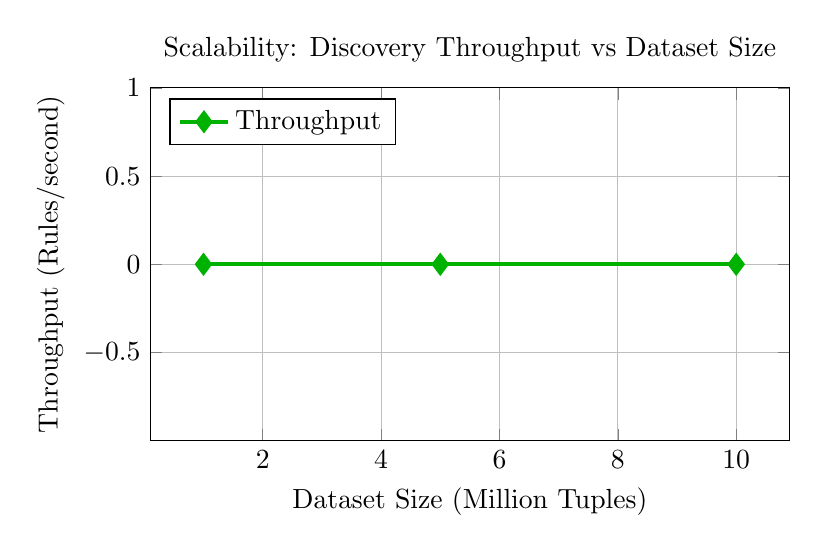
\begin{tikzpicture}
\begin{axis}[
    width=0.8\textwidth,
    height=0.5\textwidth,
    xlabel={Dataset Size (Million Tuples)},
    ylabel={Throughput (Rules/second)},
    title={Scalability: Discovery Throughput vs Dataset Size},
    grid=major,
    legend pos=north west,
    ymajorgrids=true,
    xmajorgrids=true,
    mark size=3pt,
]

% Throughput data
\addplot[
    color=green!70!black,
    mark=diamond*,
    line width=1.5pt,
] coordinates {
    (1.0,0.00)
    (5.0,0.00)
    (10.0,0.00)
};
\addlegendentry{Throughput}

\end{axis}
\end{tikzpicture}


\subsection{Overview}

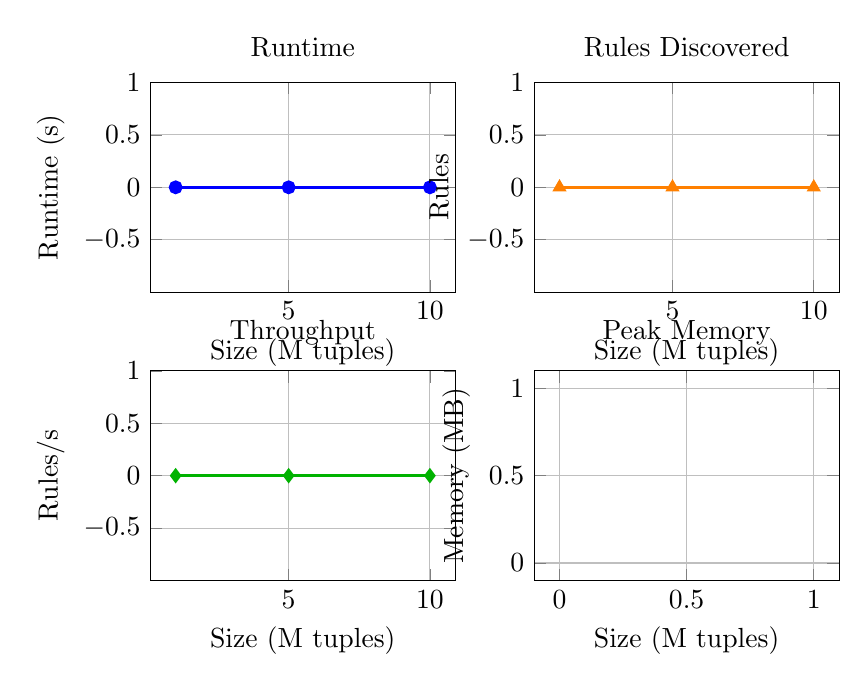
\begin{tikzpicture}

% Runtime (top-left)
\begin{axis}[
    name=runtime,
    width=0.45\textwidth,
    height=0.35\textwidth,
    xlabel={Size (M tuples)},
    ylabel={Runtime (s)},
    title={Runtime},
    grid=major,
    mark size=2pt,
]
\addplot[color=blue, mark=*, line width=1pt] coordinates {
    (1.0,0.00)
    (5.0,0.00)
    (10.0,0.00)
};
\end{axis}

% Rules (top-right)
\begin{axis}[
    name=rules,
    at={($(runtime.east)+(1cm,0)$)},
    anchor=west,
    width=0.45\textwidth,
    height=0.35\textwidth,
    xlabel={Size (M tuples)},
    ylabel={Rules},
    title={Rules Discovered},
    grid=major,
    mark size=2pt,
]
\addplot[color=orange, mark=triangle*, line width=1pt] coordinates {
    (1.0,0)
    (5.0,0)
    (10.0,0)
};
\end{axis}

% Throughput (bottom-left)
\begin{axis}[
    name=throughput,
    at={($(runtime.south)-(0,1cm)$)},
    anchor=north,
    width=0.45\textwidth,
    height=0.35\textwidth,
    xlabel={Size (M tuples)},
    ylabel={Rules/s},
    title={Throughput},
    grid=major,
    mark size=2pt,
]
\addplot[color=green!70!black, mark=diamond*, line width=1pt] coordinates {
    (1.0,0.00)
    (5.0,0.00)
    (10.0,0.00)
};
\end{axis}

% Memory or Scaling factor (bottom-right)
\begin{axis}[
    name=memory,
    at={($(throughput.east)+(1cm,0)$)},
    anchor=west,
    width=0.45\textwidth,
    height=0.35\textwidth,
    xlabel={Size (M tuples)},
    ylabel={Memory (MB)},
    title={Peak Memory},
    grid=major,
    mark size=2pt,
]
\end{axis}

\end{tikzpicture}


\section{Scalability Metrics}

\begin{itemize}
    \item Average Scaling Factor: 0.00
    \item Interpretation: sub-linear
\end{itemize}

\textbf{Interpretation:}
\begin{itemize}
    \item $< 1.0$ = Sub-linear (excellent scaling)
    \item $\approx 1.0$ = Linear (good scaling)
    \item $> 1.0$ = Super-linear (poor scaling)
\end{itemize}


\end{document}
